\chapter{Reinforcement learning}
\label{chap-reinforcement}

So far, all the learning problems we have looked at have been {\em supervised}, that is, for each training input $\ex{x}{i}$, we
are told which value $\ex{y}{i}$ should be the output. {\em Reinforcement learning}\index{reinforcement learning} differs from previous learning problems in several important ways:

% \note{We also looked at Markov Decision Processes; but in that setting, we do not \emph{learn} anything based on any data. Instead, the whole process is fully defined.}

\begin{itemize}
  \item The learner interacts explicitly with an environment, rather
        than implicitly (as in supervised learning) through an available
        training data set of $(\ex{x}{i}, \ex{y}{i})$ pairs drawn from the
        environment.
  \item The learner has some choice over what new information it
        seeks to gain from the environment.
  \item The learner updates models incrementally \note{{\em Online
              learning} is a variant of supervised learning in which new data
          pairs become available over time and the model is updated, e.g., by
          retraining over the entire larger data set, or by weight update
          using just the new data.} as additional information about the
        environment becomes available.
\end{itemize}

In a reinforcement learning problem, the interaction with the
environment takes a particular form:
\begin{center}
  \begin{tikzpicture}[main node/.style={draw,rounded corners,font=\Large},
      arr/.style={->, thick, shorten <=5pt, shorten >=5pt,}]
    \node[main node] (rl) at (0,1) {Learner};
    \node[main node] (env) at (0,-1) {Environment};
    \draw (env.west) edge[arr, bend left=50, looseness=1.1]
    node[right] {reward} ($(rl.west) + (0, -0.1)$);
    \draw ($(env.west) + (0,-0.1)$) edge[arr, bend left=70, looseness=1.5]
    node[left] {state} ($(rl.west) + (0, 0.1)$);
    \draw (rl.east) edge[arr, bend left=70, looseness=1.5]
    node[right] {action} (env.east);
  \end{tikzpicture}
\end{center}
\begin{compactitem}
  \item Learner observes {\em input} state $\ex{s}{i}$
  \item Learner generates {\em output} action $\ex{a}{i}$
  \item Learner observes {\em reward} $\ex{r}{i}$
  \item Learner observes {\em input} state $\ex{s}{i+1}$
  \item Learner generates {\em output} action $\ex{a}{i+1}$
  \item Learner observes {\em reward} $\ex{r}{i+1}$
  \item $\ldots$
\end{compactitem}

Similar to MDPs, the learner is supposed to find a {\em policy}\index{reinforcement
  learning!policy}\index{policy!reinforcement learning}, mapping a state $s$
to action $a$, that maximizes expected reward over time.

%% \question{Suppose you have the entire history of $(\ex{s}{i},
%%   \ex{a}{i}, \ex{r}{i})$ tuples from previous interactions with
%%   the environment. Could you use supervised learning to build a model
%%   that takes input (state) $s$ and predicts output (preferred action)
%%   $a$? What assumptions might be needed?}


% This problem setting is equivalent to {\em online} supervised
% learning under the following assumptions:
% \begin{enumerate}
%   \item The space of possible outputs is binary
%         (e.g., $\{+1, -1\}$) and the space of possible rewards is binary
%         (e.g., $\{+1, -1\}$);
%   \item $\ex{s}{i}$ is independent of all previous $\ex{s}{j}$ and
%         $\ex{a}{j}$; and
%   \item $\ex{r}{i}$ depends only on $\ex{s}{i}$ and $\ex{a}{i}$.
% \end{enumerate}
% In this
% case, for any experience tuple $(\ex{s}{i}, \ex{a}{i}, \ex{r}{i})$, we
% can generate a supervised training example, which is equal to
% $(\ex{s}{i}, \ex{a}{i})$ if $\ex{r}{i} = +1$ and $(\ex{s}{i},
%   -\ex{a}{i})$ otherwise.
% \question{What supervised-learning loss function would this objective
%   correspond to?}

% Markov decision processes ({\sc mdp}s) form a more general and
% flexible basis for reinforcement learning.  We began in
% Section~\ref{sec-finding_mdp_policies} with a discussion of how to
% find optimal policies for {\sc mdp}s when the {\sc mdp} is completely
% known in advance.  However, in many scenarios, full information about
% the {\sc mdp} is unavailable.  For example, consider the case when the
% above three assumptions do not hold.  When we relax assumption 1
% above, we have the class of {\em bandit problems}\index{bandit
%   problem}, which we discuss in Section~\ref{sec-bandit}.  If we relax
% assumption 2, but assume that the environment that the agent is
% interacting with is an {\sc mdp}, so that $\ex{s}{i}$ depends only on
% $\ex{s}{i-1}$ and $\ex{a}{i-1}$ then we are in the classical {\em
%     reinforcement-learning} setting, which we discuss in
% Section~\ref{rl}.  Weakening the assumptions further, for instance,
% not allowing the learner to observe the current state completely and
% correctly, makes the problem into a {\em partially observed
%     MDP}\index{Markov decision policy!partially observed MDP} ({\sc
%   pomdp}), which is substantially more difficult, and beyond the scope
% of this class.


\section{Reinforcement learning algorithms overview}
\label{rl}

A {\em reinforcement learning ({\sc rl})
    algorithm}\index{reinforcement learning!RL algorithm} is a kind of a
policy that depends on the whole history of states, actions, and
rewards and selects the next action to take. There are several
different ways to measure the quality of an {\sc rl} algorithm,
including:
\begin{itemize}
  \item Ignoring the $r^{(i)}$ values that it gets {\em while} learning,
        but considering how many interactions with the environment are
        required for it to learn a policy $\pi: \mathcal{S} \rightarrow
          \mathcal{A}$ that is nearly optimal.
  \item Maximizing the expected sum of discounted rewards while
        it is learning.
\end{itemize}
Most of the focus is on the first criterion (which is called ``sample efficiency''), because the second one is
very difficult.  The first criterion is reasonable when the learning
can take place somewhere safe (imagine a robot learning, inside the
robot factory, where it can't hurt itself too badly) or in a simulated
environment.

Approaches to reinforcement learning differ significantly according to
what kind of hypothesis or model is being learned. Roughly speaking, RL
methods can be categorized into model-free methods and model-based
methods. 
The main distinction is that model-based methods explicitly
learn the transition and reward models to assist the end-goal of
learning a policy; model-free methods do not.  We will start our discussion with the model-free
methods, and introduce two of the arguably most popular types of algorithms,
Q-learning (Section~\ref{sec-q_learning}) and policy gradient
(Section~\ref{sec-rl_policy_search}).  We then describe
model-based methods (Section~\ref{sec-rl_model_based}). Finally, we
briefly consider ``bandit'' problems (Section~\ref{sec-bandit}), which differ
from our {\sc mdp} learning context by having probabilistic rewards.




%%%%%%%%%%%%%%%%%%%%
\section{Model-free methods}

Model-free methods are methods that do not explicitly learn transition
and rewards models. Depending on what is explicitly being learned,
model-free methods are sometimes further categorized into value-based
methods (where the goal is to learn/estimate a value function)
% (where value is a shorthand for value functions) 
and
policy-based methods (where the goal is to directly learn an optimal policy). It's important to note that such
categorization is approximate and the boundaries are blurry. In fact,
current RL research tends to combine the learning of value functions,
policies, and transition and reward models all into a complex learning
algorithm, in an attempt to combine the strengths of each approach.


% --e.g., in (tabular) Q-learning (Section \ref{sec-q_learning}) right
% below, the Machine Learning model used is a table. We will soon see
% other (ML) models used in the model-free methods, such as neural
% networks.


\subsection{Q-learning}\label{sec-q_learning}
Q-learning is a frequently used class of RL algorithms that
concentrates on learning (estimating) the state-action value function, i.e.,
the $Q$ function. Specifically, recall the {\sc mdp} value-iteration update:
\note{The thing that most students seem to get confused about is when
  we do value iteration and when we do Q learning.  Value iteration
  assumes you know $T$ and $R$ and just need to {\em compute} $Q$.  In
  $Q$ learning, we don't know or even directly estimate $T$ and $R$:
  we estimate $Q$ directly from experience!}
\begin{equation}
  Q(s,a) = R(s,a) + \gamma \sum_{s'} T(s,a,s')\max_{a'}Q(s',a')
\end{equation}
The Q-learning algorithm below adapts this value-iteration idea to the
  {\sc rl} scenario, where we do not know the transition function $T$ or
reward function $R$, and instead rely on samples to perform the updates.
\begin{codebox}
  \Procname{$\proc{Q-Learning}(\mathcal{S}, \mathcal{A},  \gamma, \alpha, s_0, \text{max-iter})$}\label{proc:Q_learn}
  \li $i=0$ 
  \li \For $s \in \mathcal{S}, a \in \mathcal{A}:$
  \li   \Do
  ${Q_{old}}(s, a) = 0$
  \End
  \li $s \gets s_0$
  \li \While $i < \text{max-iter}$:
  \li \Do
  $a \gets \text{select}\_\text{action}(s, {Q_{old}}(s, a))$
  \li     $r,s' \gets \text{execute}(a)$
  \li     ${Q}_{\text{new}}(s, a) = (1-\alpha){Q}_{\text{old}}(s, a)
    + \alpha(r + \gamma \max_{a'}{Q}_{\text{old}}(s', a'))$
  \li $s \gets s'$
  \li $i \gets (i+1)$
  \li      $Q_{\text{old}} = Q_{\text{new}}$
  \End
  \li \Return $Q_{\text{new}}$
  \End
\end{codebox}

With the pseudo-code provided for \nameref{proc:Q_learn}, there are a few
key things to note. First, we must determine which state to initialize the
learning from. In the context of a game, this initial state may be well defined.
In the context of a robot navigating an environment, one may consider
sampling the initial state at random. In any case, the initial state is necessary
to determine the trajectory the agent will experience as it navigates the environment.
Second, different contexts will influence how we want to choose when to stop
iterating through the while loop. Again, in some games there may be a clear
terminating state based on the rules of how it is played. On the other hand,
a robot may be allowed to explore an environment \emph{ad infinitum}.
In such a case, one may consider either setting a fixed number of transitions (as done explictly in the pseudo-code) to take; or we may want to stop iterating in the example once the values in the Q-table are not changing, after the algorithm has been running for a while. Finally, a single trajectory through the environment may not be sufficient to adequately explore all state-action pairs. In these instances, it becomes necessary to run
through a number of iterations of the \nameref{proc:Q_learn} algorithm, potentially
with different choices of initial state $s_0$\note{This notion of running a number
  of instances of \nameref{proc:Q_learn} is often referred to as experiencing multiple
  \emph{episodes}.}. Of course, we would then want to modify \nameref{proc:Q_learn} such
that the Q table is not reset with each call.

Now, let's dig in to what is happening in \nameref{proc:Q_learn}.
Here, $\alpha\in (0,1]$ represents the ``learning rate,'' which needs to decay
for convergence purposes, but in practice is often set to a
constant. It's also worth mentioning that Q-learning assumes a
discrete state and action space where states and actions take on
discrete values like $1,2,3,\dots$ etc. In contrast, a continuous
state space would allow the state to take values from, say, a
continuous range of numbers; for example, the state could be any real
number in the interval $[1,3]$. Similarly, a continuous action space
would allow the action to be drawn from, e.g., a continuous range of
numbers. There are now many extensions developed based on Q-learning
that can handle continuous state and action spaces (we'll look at one
soon), and therefore the algorithm above is also sometimes referred to
more  specifically as tabular Q-learning.

In the Q-learning update rule
\begin{equation}\label{q_avg}
  Q[s, a] \leftarrow (1-\alpha)Q[s, a]
  + \alpha(r + \gamma \max_{a'}Q[s',a'])
\end{equation}
the term $r + \gamma \max_{a'} Q[s',a']$ is often referred to as the
(one-step look-ahead) \emph{target}. The update can be viewed as a
combination of two different iterative processes that we have already
seen: the combination of an old estimate with the target using a
running average with a learning rate $\alpha$, and the
dynamic-programming update of a $Q$ value from value iteration.


Eq.~\ref{q_avg} can also be equivalently rewritten as
\begin{equation}\label{td:q}
  Q[s, a] \leftarrow Q[s, a]
  + \alpha\left((r + \gamma \max_{a'}
  Q[s',a'])-Q[s,a]\right),
\end{equation}
which allows us to interpret Q-learning in yet another way: we make an
update (or correction) based on the temporal difference between the
target and the current estimated value $Q[s, a].$


% It is actually not a gradient update, but later, when we consider
% function approximation, we will treat it as if it were.}

% And besides an "almost" gradient interpretation, writing the
% Q-learning update rule in (\ref{td:q}) form also allows us to make
% a connection to a whole family of sampling-based reinforcement
% learning methods called {\em temporal difference} (TD) learning
% method\index{reinforcement learning!temporal difference method}. TD
% methods are so-named


The Q-learning algorithm above includes a procedure called {\it select\_action},
that, given the current state $s$ and current $Q$ function, has to decide
which action to take.  If the $Q$ value is estimated very accurately
and the agent is behaving in the world, then generally we would want
to choose the apparently optimal action $\argmax{a \in \mathcal{A}}
  Q(s,a)$.  But, during learning, the $Q$ value estimates won't be very
good and exploration is important.  However, exploring completely at
random is also usually not the best strategy while learning, because
it is good to focus your attention on the parts of the state space
that are likely to be visited when executing a good policy (not a bad
or random one).

A typical action-selection strategy that attempts to address this
  {\em exploration versus exploitation} dilemma is the so-called {\em
$\epsilon$-greedy} strategy:
\begin{itemize}
  \item with probability $1-\epsilon$, choose
        $\argmax{a \in \mathcal{A}} Q(s,a)$;
  \item with probability $\epsilon$, choose the action $a \in \mathcal{A}$
        uniformly at random.
\end{itemize}
where the $\epsilon$ probability of choosing a random action helps the
agent to explore and try out actions that might not seem so desirable
at the moment.


Q-learning has the surprising property that it is {\em guaranteed} to
converge to the actual optimal $Q$ function under fairly weak
conditions!  Any exploration strategy is okay as long as it tries
every action infinitely often on an infinite run (so that it doesn't
converge prematurely to a bad action choice).

Q-learning can be very inefficient. Imagine a robot that has a
choice between moving to the left and getting a reward of 1, then
returning to its initial state, or moving to the right and walking
down a 10-step hallway in order to get a reward of 1000, then
returning to its initial state.

\begin{center}
  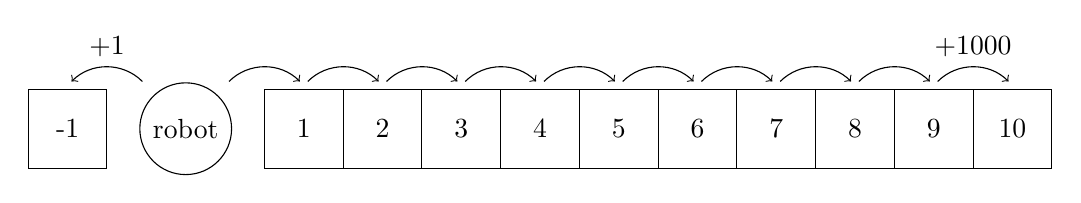
\begin{tikzpicture}
    \draw (-3,0) grid (-2,1);
    \draw (0,0) grid (10,1);
    \node[circle, draw] (robot) at (-1,.5) {robot};
    % right arrows
    \foreach \x in {1,2,3,4,5,6,7,8,9,10} {
        \coordinate (a) at (\x - 1.45, 1.1);
        \coordinate (b) at (\x - .55, 1.1);
        \draw (a) edge[->, bend left=45] coordinate (mid) (b);
        \node at (\x - .5, .5) {\x};
      }
    \node[above] (reward) at (mid) {+1000};

    % left arrow
    \coordinate (a) at (-2.45, 1.1);
    \coordinate (b) at (-1.55, 1.1);
    \draw (b) edge[->, bend right=45] node[above] {+1} (a);
    \node at (-2.5, .5) {-1};
  \end{tikzpicture}
\end{center}

The first time the robot moves to the right and goes down the hallway,
it will update the $Q$ value just for state 9 on the hallway and
action ``right'' to have a high value, but it won't yet understand
that moving to the right in the earlier steps was a good choice. The
next time it moves down the hallway it updates the value of the state
before the last one, and so on.  After 10 trips down the hallway, it
now can see that it is better to move to the right than to the left.

\setcounter{MaxMatrixCols}{20}

More concretely, consider the vector of Q values $Q(i = 0, \ldots, 9;
  \text{right})$, representing the Q values for moving right at each of
the positions $i = 0, \ldots, 9$. Position index $0$ is the starting
position of the robot as pictured above.

Then, for $\alpha=1$ and $\gamma = 0.9$, Eq.~\ref{td:q} becomes
\begin{equation}
  Q(i, \text{ right}) = R(i, \text{ right})
  + 0.9 \cdot \max_a Q(i+1, a).
\end{equation}
Starting with Q values of 0,
\begin{equation}
  Q^{(0)}(i = 0, \ldots, 9; \text{ right}) =
  \begin{bmatrix} 0 & 0 & 0 & 0 & 0 & 0 & 0 & 0 & 0 & 0 \end{bmatrix}.
\end{equation}
\note{We are violating our usual notational conventions here, and
  writing $\ex{Q}{i}$ to mean the Q value function that results after
  the robot runs all the way to the end of the hallway, when executing
  the policy that always moves to the right.}  Since the only nonzero
reward from moving right is $R(9, \text{ right}) = 1000$, after our
robot makes it down the hallway once, our new Q vector is
\begin{equation}
  Q^{(1)}(i = 0, \ldots, 9; \text{ right}) =
  \begin{bmatrix} 0 & 0 & 0 & 0 & 0 & 0 & 0 & 0 & 0 & 1000 \end{bmatrix}.
\end{equation}
After making its way down the hallway again,
$Q(8, \text{ right}) = 0 + 0.9 \cdot Q(9, \text{ right}) = 900$
updates:
\begin{equation}
  Q^{(2)}(i = 0, \ldots, 9; \text{ right}) =
  \begin{bmatrix}
    0 & 0 & 0 & 0 & 0 & 0 & 0 & 0 & 900 & 1000
  \end{bmatrix}.
\end{equation}
Similarly,
\begin{align}
  Q^{(3)}(i = 0, \ldots, 9; \text{ right})   & =
  \begin{bmatrix}
    0 & 0 & 0 & 0 & 0 & 0 & 0 & 810 & 900 & 1000
  \end{bmatrix}                 \\
  Q^{(4)}(i = 0, \ldots, 9; \text{ right})   & =
  \begin{bmatrix}
    0 & 0 & 0 & 0 & 0 & 0 & 729 & 810 & 900 & 1000
  \end{bmatrix}               \\
                                             & \vdotswithin{=} \\
  Q^{(10)}(i = 0, \ldots, 9;  \text{ right}) & =
  \begin{bmatrix}
    387.4 & 420.5 & 478.3 & 531.4 & 590.5 & 656.1 & 729 & 810
          & 900   & 1000
  \end{bmatrix},
\end{align}
and the robot finally sees the value of moving right from position 0.
\note{Here, we can see the exploration/exploitation dilemma in action: from the perspective of $s_0=0$, it
  will seem that getting the immediate reward of $1$
  is a better strategy without exploring the long hallway.}
\question{Determine the Q value functions that will result from updates due to the robot always executing the ``move left'' policy.}


\subsection{Function approximation: Deep Q learning}
In our Q-learning algorithm above, we essentially keep track of each
$Q$ value in a table, indexed by $s$ and $a$. What do we do if
$\mathcal{S}$ and/or $\mathcal{A}$ are large (or continuous)?

We can use a function approximator like a neural network to store Q
values. For example, we could design a neural network that takes in
inputs $s$ and $a$, and outputs $Q(s,a)$. We can treat this as a
regression problem, optimizing this loss\note{This is the so-called
  squared Bellman error; as the name suggests, it's closely related to
  the Bellman equation we saw in {\sc mdp}s in Chapter~\ref{chap-mdps}.
  Roughly speaking, this error measures how much the
  Bellman equality is violated.}:
\begin{equation}
  \left(Q(s,a) - (r + \gamma \max_{a'}Q(s',a'))\right)^2\;\;,
\end{equation}
where $Q(s, a)$ is now the output  of the neural network.

There are several different architectural choices for using a
neural network to approximate $Q$ values:
\begin{itemize}
  \item One network for each action $a$, that takes $s$ as input and
        produces $Q(s, a)$ as output;
  \item One single network that takes $s$ as input and produces a vector
        $Q(s, \cdot)$, consisting of the $Q$ values for each action; or
  \item One single network that takes $s, a$ concatenated into a vector
        (if $a$ is discrete, we would probably use a one-hot encoding,
        unless it had some useful internal structure) and produces $Q(s, a)$
        as output.
\end{itemize}

\note{For continuous action spaces, it is popular to use
  a class of methods called {\em actor-critic}
  methods\index{reinforcement!actor-critic methods}, which combine
  policy and value-function learning.  We won't get into them in
  detail here, though.}

The first two choices are only suitable for discrete (and not too big)
action sets.  The last choice can be applied for continuous actions,
but then it is difficult to find $\argmax{a \in \mathcal{A}} Q(s, a)$.

There are not many theoretical guarantees about Q-learning with
function approximation and, indeed, it can sometimes be fairly
unstable (learning to perform well for a while, and then getting
suddenly worse, for example).  But neural network Q-learning has also
had some significant successes.

One form of instability that we do know how to guard against is {\em
    catastrophic forgetting.}  In standard supervised learning, we
expect that the training $x$ values were drawn independently from some
distribution. \note{And, in fact, we routinely shuffle their order in
  the data file, anyway.}  But when a learning agent, such as a robot,
is moving through an environment, the sequence of states it encounters
will be temporally correlated. For example, the robot might spend 12
hours in a dark environment and then 12 in a light one.  This can mean
that while it is in the dark, the neural-network weight-updates will
make the $Q$ function ``forget'' the value function for when it's
light.

One way to handle this is to use $\emph{experience
    replay}$\index{experience replay}, where we save our $(s,a,s',r)$
experiences in a {\it replay buffer}.  Whenever we take a step in the
world, we add the $(s,a,s',r)$ to the replay buffer and use it to do a
Q-learning update.  Then we also randomly select some number of tuples
from the replay buffer, and do Q-learning updates based on them, as
well.  In general it may help to keep a {\em sliding
    window}\index{sliding window} of just the 1000 most recent
experiences in the replay buffer.  (A larger buffer will be necessary
for situations when the optimal policy might visit a large part of the
state space, but we like to keep the buffer size small for memory
reasons and also so that we don't focus on parts of the state space
that are irrelevant for the optimal policy.)  The idea is that it will
help us propagate reward values through our state space more
efficiently if we do these updates. We can see it as doing something
like value iteration, but using samples of experience rather than a
known model.

\subsection{Fitted Q-learning}
An alternative strategy for learning the $Q$ function that is somewhat
more robust than the standard $Q$-learning algorithm is a method
called {\em fitted Q}.\index{fitted Q-learning}

\begin{codebox}
  \Procname{$\proc{Fitted-Q-Learning}(\mathcal{A}, s_0, \gamma, \alpha,
      \epsilon, m)$}
  \li $s \gets s_0$ \Comment (e.g., $s_0$ can be drawn randomly from $\mathcal{S}$)
  \li $\mathcal{D} = \{\;\}$
  \li initialize neural-network representation of $Q$
  \li \While True: \Do
  \li  $\mathcal{D}_\text{new}$ = experience from executing $\epsilon$-greedy policy based
  on $Q$ for $m$ steps
  \li $\mathcal{D} = \mathcal{D} \cup \mathcal{D}_\text{new}$ represented
  as $(s, a, s', r)$ tuples
  \li $\mathcal{D}_\text{supervised} = \{(\ex{x}{i}, \ex{y}{i})\}$  where $\ex{x}{i} =
    (s, a)$ and $\ex{y}{i} = r + \gamma \max_{a' \in \mathcal{A}} Q(s', a')$
  \li \;\;\;for each tuple $\ex{(s, a, s', r)}{i} \in \mathcal{D}$
  \li re-initialize neural-network representation of $Q$
  \li $Q = \proc{supervised-NN-regression}(\mathcal{D}_\text{supervised})$
  \End
\end{codebox}

Here, we alternate between using the policy induced by the current $Q$
function to gather a batch of data $\mathcal{D}_\text{new}$, adding it
to our overall data set $\mathcal{D}$, and then using supervised
neural-network training to learn a representation of the $Q$ value
function on the whole data set.  This method does not mix the
dynamic-programming phase (computing new $Q$ values based on old ones)
with the function approximation phase (supervised training of the
neural network) and avoids catastrophic forgetting.  The regression
training in line 10 typically uses squared error as a loss function and
would be trained until the fit is good (possibly measured on held-out
data).


%%%%%%%%%%%%%%%%%%%%


\subsection{Policy gradient}
\label{sec-rl_policy_search}

A different model-free strategy is to search directly for a good
policy.  The strategy here is to define a functional form $f(s;\theta)
  = a$ for the policy, where $\theta$ represents the parameters we learn
from experience. We choose $f$ to be differentiable, and often define \note{This
  means the chance of choosing an action depends on which state
  the agent is in. Suppose, e.g., a robot is trying to get to a
  goal and can go left or right. An unconditional policy can say: I go left 99\% of the time; a
  conditional policy can consider the robot's
  state, and say: if I'm to the right of the goal, I go left 99\% of the time.}
$f(s, a;\theta) = Pr(a|s)$, a conditional probability distribution over
our possible actions.

Now, we can train the policy parameters using gradient descent:
\begin{itemize}
  \item When $\theta$ has relatively low dimension, we can compute a
        numeric estimate of the gradient by running the policy multiple
        times for different values of $\theta$, and computing the
        resulting rewards.
  \item When $\theta$ has higher dimensions (e.g., it represents the
        set of parameters in a complicated neural network), there are more
        clever algorithms, e.g., one called {\sc REINFORCE}, but they can
        often be difficult to get to work reliably.
\end{itemize}

Policy search is a good choice when the policy has a simple known
form, but the {\sc mdp} would be much more complicated to estimate.


%%%%%%%%%%%%%%%%%%%%%%%%%%%%%%%%%%%%%%%%%%%%%%%%%%%%%%%%%%%%%%%%%%%%%%%%%%%%%


\section{Model-based RL}
\label{sec-rl_model_based}

The conceptually simplest approach to {\sc rl} is to model $R$ and $T$
from the data we have gotten so far, and then use those models,
together with an algorithm for solving {\sc mdp}s (such as value
iteration) to find a policy that is near-optimal given the current
models.

Assume that we have had some set of interactions with the environment,
which can be characterized as a set of tuples of the form $(\ex{s}{t},
  \ex{a}{t}, \ex{s}{t+1}, \ex{r}{t})$.

Because the transition function ${T}(s, a, s')$ specifies
probabilities, multiple observations of $(s, a, s')$ may be needed to
model the transition function.  One approach to this task of building
a model $\hat{T}(s, a, s')$ for the true ${T}(s,a,s')$ is to estimate
it using a simple counting strategy,
\begin{equation}
  \hat{T}(s,a,s') = \frac{\#(s,a,s') + 1}{\#(s,a) + \left|
    \mathcal{S}\right|}
  \,.
\end{equation}
Here, $\#(s, a, s')$ represents the number of times in our data set we
have the situation where $\ex{s}{t} = s, \ex{a}{t} = a, \ex{s}{t+1} =
  s'$ and $\#(s, a)$ represents the number of times in our data set we
have the situation where $\ex{s}{t} = s, \ex{a}{t} = a$.  \question{Prove to
  yourself that $\#(s,a) = \sum_{s'} \#(s,a,s')$.}

Adding 1 and $\left|\mathcal{S}\right|$ to the numerator and
denominator, respectively, are a form of smoothing called the {\em
    Laplace correction}\index{reinforcement learning!Laplace
  correction}. It ensures that we never estimate that a probability is
0, and keeps us from dividing by 0.  \note{Conceptually, this is also similar to having ``initialized'' our estimate for the transition function with uniform random probabilities, before having made any observations.} As the amount of data we gather
increases, the influence of this correction fades away.

In contrast, the reward function ${R}(s, a)$\index{reward function}
(as we have specified it in this text) is a {\em deterministic}
function, such that knowing the reward $r$ for a given $(s, a)$ is
sufficient to fully determine the function at that point.  In other
words, our model $\hat{R}$ can simply be a record of observed rewards,
such that $\hat{R}(s, a) = r = R(s,a)$.

%% A more general case is when the reward function is {\em
%%   non-deterministic}, such that the reward $R(s, a)$ may vary with
%% each query.  In this case, an estimation strategy similar to that
%% employed for the model $\hat{T}$ could be used for building the model
%% $\hat{R}$, e.g.:
%% \begin{equation}
%%   \hat{R}(s,a) = \frac{\sum r \mid s, a}{\#(s,a)}
%% \end{equation}
%% where
%% \begin{equation}
%%   \sum r \mid s, a = \sum_{\{t \mid \ex{s}{t} = s, \ex{a}{t} = a\}}
%%   \ex{r}{t}\;\;.
%% \end{equation}
%% Such an estimate would just be the average of the observed rewards for
%% each $s, a$ pair.  However, this general case is outside the scope of
%% what we cover here.

Given empirical models $\hat{T}$ and $\hat{R}$ for the transition and
reward functions, we can now solve the {\sc mdp} $(\mathcal{S},
  \mathcal{A}, \hat{T}, \hat{R})$ to find an optimal policy using value
iteration, or use a search algorithm to find an action
to take for a particular state.

This approach is effective for problems with small state and action
spaces, where it is not too hard to get enough experience to model $T$
and $R$ well; but it is difficult to generalize this method to handle
continuous (or very large discrete) state spaces, and is a topic of
current research.

% \section{Applications}
% \subsection{Atari games}
% \begin{itemize}
%   \item Input(s): 4 downsampled screen images (recent frames)
%   \item Output: discrete joystick command
%   \item Q-learning + experience replay + NN
%   \item Surprisingly effective, but
%     \begin{itemize}
%       \item not good at long-term planning ($\gamma = 0.99$)
%       \item not good when partially observable
%     \end{itemize}
% \end{itemize}
% \subsection{AlphaZero}
% Two player zero-sum complete information games can be solved using
% (a minor variant of) value iteration. It takes advantage of the fact
% that $V(s)$ for player 1 is basically $-V(s)$ for player 2.
%
% Q-learning works, too.
% \begin{description}
%   \item[1992:] TD-Gammon learns to play Backgammon at near expert
%     level. Uses hand-crafted board features $\phi(s)$ as input to
%     a neural network, trained with 1.5 million games of self play.
%   \item[2017:] Silver et al. use similar ideas at a much larger
%     scale in AlphaZero, and use a tree search to improve value
%     estimates and generate supervised training data.
%
%     AlphaZero learns to play Go, chess, and Shogi as well or better
%     than the best computer players.
% \end{description}


%%%%%%%%%%%%%%%%%%%%%%%%%%%%%%%%%%%%%%%%%%%%%%%%%%%%%%%%%%%%%%%%%%%%%%%%%%%%%

\section{Bandit problems}
\label{sec-bandit}

Bandit problems differ from our reinforcement learning setting as
described above in two ways: the reward function is probabilistic, and
the key decision is usually framed as whether or not to continue
exploring (to improve the model) versus exploiting (take actions to
maximize expected rewards based on the current model).

A basic bandit problem is given by
\begin{itemize}
  \item A set of actions $\mathcal{A}$;
  \item A set of reward values $\mathcal{R}$; and
  \item A probabilistic reward function $R_p: {\mathcal{A}} \times
          {\mathcal{R}} \rightarrow \mathbb{R}$, i.e., $R_p$ is a function that
        takes an action and a reward and returns the probability of getting
        that reward conditioned on that action being taken, $R_p(a, r) =
          Pr({\rm reward} = r \, |\, {\rm action} = a)$.  This is analogous to
        how the transition function $T$ is defined.  Each time the agent
        takes an action, a new value is drawn from this distribution.
\end{itemize}

The most typical bandit problem has $\mathcal{R} = \{0, 1\}$ and
$\lvert \mathcal{A} \rvert = k$.  This is called a {\em $k$-armed
    bandit problem}\index{bandit problem!k-armed bandit}\note{Why?
  Because in English slang, ``one-armed bandit'' is a name for a slot
  machine (an old-style gambling machine where you put a coin into a
  slot and then pull its arm to see if you get a payoff) because it
  has one arm and takes your money!  What we have here is a similar
  sort of machine, but with $k$ arms.}, where the decision is which
``arm'' (action $a$) to select, and the reward is either getting a
payoff ($1$) or not ($0$).  There is a lot of mathematical literature
on optimal strategies for $k$-armed bandit problems under various
assumptions.  The important question is usually one of {\em
    exploration versus exploitation}\index{reinforcement
  learning!exploration vs. exploitation}.  Imagine that you have tried
each action 10 times, and now you have estimates $\hat{R}_p(a, r)$ for
the probabilities $R_p(a, r)$ for reward $r$ given action $a$.  Which
arm should you pick next?  You could
\begin{description}
  \item{\bf exploit} your knowledge, and for future trials choose the
        arm with the highest value of expected reward; or
  \item{\bf explore} further, by trying some or all actions more times,
        hoping to get better estimates of the $R_p(a, r)$ values.
\end{description}
The theory ultimately tells us that, the longer our horizon $h$ (or,
similarly, closer to $1$ our discount factor), the more time we should
spend exploring, so that we don't converge prematurely on a bad choice
of action.
\question{Why is it that ``bad'' luck during exploration is more
  dangerous than ``good'' luck?  Imagine that there is an action that
  generates reward value 1 with probability 0.9, but the first three
  times you try it, it generates value 0.  How might that cause
  difficulty?  Why is this more dangerous than the situation when an
  action that generates reward value 1 with probability 0.1 actually
  generates reward 1 on the first three tries?  }

Bandit problems are reinforcement learning problems (and are very
different from batch supervised learning\note{There is a setting of
  supervised learning, called {\em active learning}\index{active
    learning}, where instead of being given a training set, the
  learner gets to select a value of $x$ and the environment gives back
  a label $y$; the problem of picking good $x$ values to query is
  interesting, but the problem of deriving a hypothesis from $(x, y)$
  pairs is the same as the supervised problem we have
  been studying.})  in that:
\begin{itemize}
  \item The agent gets to influence what data it obtains (selecting $a$
        gives it another sample from $R(a, r)$), and
  \item The agent is penalized for mistakes it makes while it is
        learning (if it is trying to maximize the expected
        reward $\sum_r r \cdot Pr(R_p(a, r) = r)$ it gets while behaving).
\end{itemize}

In a {\em contextual} bandit problem\index{bandit problem!contextual
  bandit problem}, you have multiple possible states, drawn from some
set $\mathcal{S}$, and a separate bandit problem associated with each
one.

Bandit problems are an essential subset of reinforcement
learning.  It's important to be aware of the issues, but we will not
study solutions to them in this class.



%%% Local Variables:
%%% mode: latex
%%% TeX-master: "top"
%%% End:
